\documentclass[pdf]{beamer}

\mode<presentation>{}

\usepackage{xcolor}

% Declare some colors

\definecolor{lightred}{HTML}{ff4b4b}
\definecolor{lightblue}{HTML}{323296}

% Theme settings

\setbeamercolor*{background canvas}{bg=black}
\setbeamercolor*{normal text}{fg=white}
\setbeamercolor*{title}{fg=white}
\setbeamercolor*{frametitle}{fg=lightred}
\setbeamercolor*{itemize item}{fg=white}

\useinnertheme{rectangles}

%% preamble
\title{Challenges of Ring}
\subtitle{contributing to the future of free communication platforms}
\author{Hugo Lefeuvre \\ \href{mailto:hle@debian.org}{\texttt{hle@d.o}}}
\begin{document}

%% title frame
\begin{frame}
\titlepage
\end{frame}

%% normal frame
\begin{frame}{What Ring is}

\begin{itemize}
\uncover<1->{\item Distributed communication platform}
\uncover<2->{\item Respects Privacy and Freedom}
\uncover<3->{\item GNU package}
\uncover<4->{\item Debian package}
\uncover<5->{\item Many platforms (Android, macOS, Windows, iOS)}
\uncover<6->{\item ... developed by \href{https://savoirfairelinux.com}{Savoir-Faire Linux}, in Montréal}
\end{itemize}

\end{frame}

%% --------------------------

\begin{frame}{What Ring does}

\begin{itemize}
\uncover<1->{\item Message chat}
\uncover<2->{\item Audio \& Video calls}
\uncover<3->{\item File transfer}
\uncover<4->{\item Video conferences}
\uncover<5->{\item SIP client: calls, forwarding !}
\end{itemize}

\end{frame}

%% --------------------------

\begin{frame}{It's all about challenges}

Pioneering = no stackoverflow or whatsoever :)

\end{frame}

%% --------------------------

\begin{frame}{It's all about challenges}

\uncover<1-1>{\texttt{eb3c27067c4637b99bf9895d5babb2c77c3115b5}

can you remember that ?}

\uncover<2->{\Large{of course not}}

\end{frame}

%% --------------------------

\begin{frame}{Name server}

providing aliases to ringID

\texttt{eb3c27067c4637b99bf9895d5babb2c77c3115b5} $\rightarrow$ \texttt{hlef}

\end{frame}

%% --------------------------
\begin{frame}{Name server}

\begin{itemize}
\uncover<1->{\item registering a name = blockchain contract on Ethereum blockchain}
\uncover<2->{\item so it is distributed, right ?}
\uncover<3->{\item it depends on the blockchain "type"}
\end{itemize}

\end{frame}

%% --------------------------

\begin{frame}{Name server}

How it works currently

\begin{itemize}
\uncover<1->{\item we can't let random people modify the name registers without supervision}
\uncover<2->{\item $\rightarrow$ consortium blockchain (restricted group of entities allowed to operate)}
\uncover<3->{\item carefully select the contributors?}
\uncover<4->{\item currently only SFL}
\uncover<5->{\item $\rightarrow$ trusted organizations ?}
\end{itemize}

\end{frame}

%% --------------------------

\begin{frame}{Emoji}

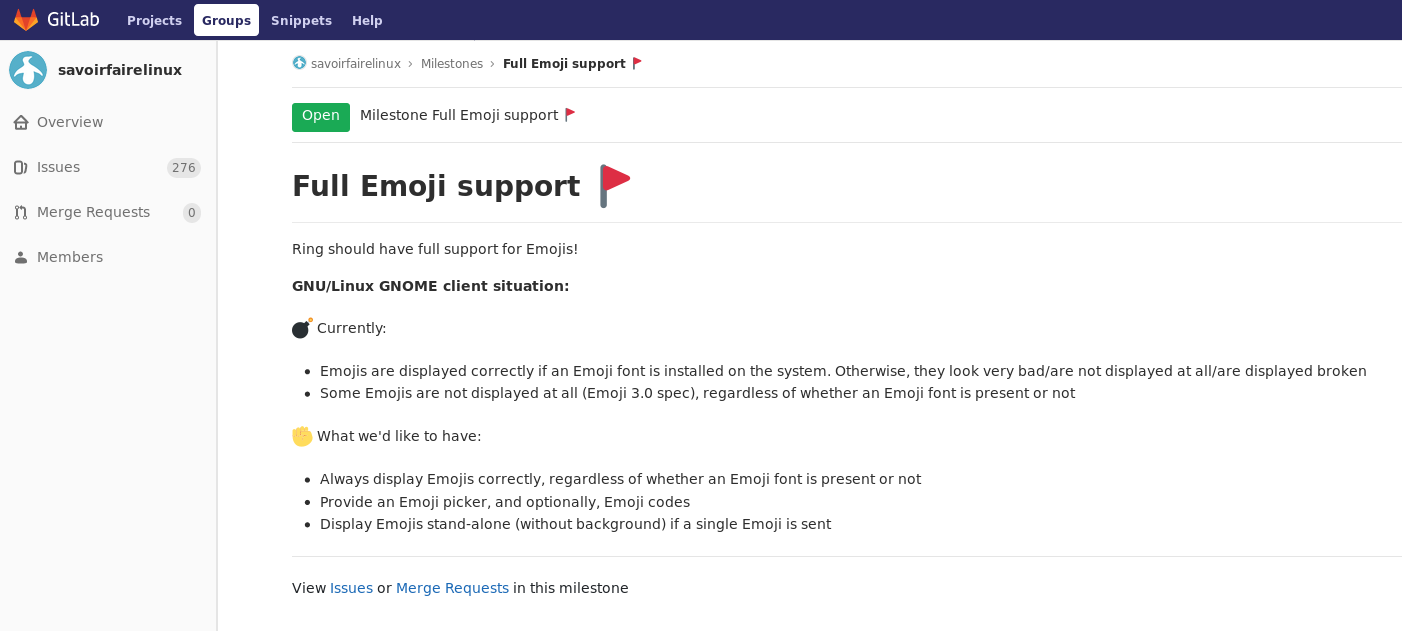
\includegraphics[height=100px]{pix/milestone-emoji.png}

\end{frame}

%% --------------------------

\begin{frame}{It's all about challenges}

\begin{itemize}
\item Offline messaging (data persistance)
\item Group chat
\item Battery on mobile devices
\item ...
\end{itemize}

\end{frame}

%% --------------------------

\begin{frame}{It's all about challenges}

but also...

\uncover<2-2>{\Large External contributors !}
\uncover<3->{
\includegraphics[height=100px]{pix/pinguin.jpg}}

\end{frame}

%% --------------------------

\begin{frame}{It's all about challenges}

not a matter of pinguins and kitten

\end{frame}

%% --------------------------

\begin{frame}{It's all about challenges}

\begin{itemize}
\item small core team, working full time on Ring
\item Gerrit code review
\item previously on Tuleap, migrated to Gitlab
\end{itemize}

\end{frame}

%% --------------------------

\begin{frame}{want to help ?}

\begin{table}
\centering
\begin{tabular}{llllll}
C/C++       & Daemon, LRC, GNOME Client \\
HTML/JS/CSS & GNOME Client chatview     \\
Java        & Android Client            \\
Networking  & PJSIP                     \\
Swift       & iOS Client                \\
ObjectiveC++& macOS Client
\end{tabular}
\end{table}

\end{frame}

%% --------------------------

\begin{frame}{Where to start ?}

\begin{itemize}
\item \href{https://ring.cx}{\texttt{ring.cx}} official website
\item \href{https://git.ring.cx}{\texttt{git.ring.cx}} Gitlab to report bugs
\item \href{https://gerrit-ring.savoirfairelinux.com}{\texttt{gerrit-ring.savoirfairelinux.com}} Gerrit to submit patches
\item \href{{mailto:ring@gnu.org}}{\texttt{ring@gnu.org}}
\item now, around a \texttt{\$beverage} :)
\end{itemize}

\end{frame}

\end{document}
